\documentclass{scrreprt}
% language
\usepackage[ngerman]{babel}
\usepackage[utf8]{inputenc}
%\usepackage{ngerman}

% color
\usepackage{xcolor}
% tables
\usepackage{tabularx}
% figures
\usepackage{graphicx}
% boxes
\usepackage{tcolorbox}
% math
\usepackage{amsmath}
% header
\usepackage{fancyhdr}
% code
\usepackage{minted}
% plots
\usepackage{pgfplots}
% bibliography
\usepackage[citestyle=authortitle-ibid]{biblatex}
% random text
\usepackage{lipsum}
% links
\usepackage{hyperref}
% glossary (must be after links)
\usepackage[toc,nonumberlist]{glossaries}

\renewcommand{\familydefault}{\sfdefault}

\pagestyle{fancy}

%%% Bibliography
\addbibresource{bibliography.bib}
%%%%%%

%%% Glossar
\makeglossaries
\loadglsentries{glossary.tex}
%%%%%%

\setminted{
    linenos=true,
}

% %%% Darkmode
% \pgfplotsset{
%     legend style={fill=black,draw=white}
%     }
% \usemintedstyle{monokai}
% \pagecolor[rgb]{0.1,0.1,0.1} %black
% \color[rgb]{0.8,0.8,0.8} %grey
% %\pagecolor[rgb]{0.0,0.0,0.0} %black
% %\color[rgb]{1,1,1} %white
% %%%


%%% Titlepage
\subject{Jannis' \LaTeX~template}
\title{Hello World!}
\date{\today}
\author{Jannis Matteo Imhof}
%%%%%%

\begin{document}
%%% sans serif font family
\maketitle

\tableofcontents

\chapter{Hello World!}
\Gls{foo}

\section{tcolorbox}
\begin{tcolorbox}[colback=red!5!white,colframe=red!75!black,title=My nice heading]
    This is another \textbf{tcolorbox}.
    \tcblower
    Here, you see the lower part of the box.
\end{tcolorbox}

\begin{tcolorbox}[colback=black!25!white,colframe=black!75!white,title=My nice heading]
    This is another \textbf{tcolorbox}.
    \tcblower
    Here, you see the lower part of the box.
\end{tcolorbox}

\begin{tcolorbox}
    This is another \textbf{tcolorbox}.
    \tcblower
    Here, you see the lower part of the box.
\end{tcolorbox}

\section{figure}
\begin{figure}[!h]
    \centering
    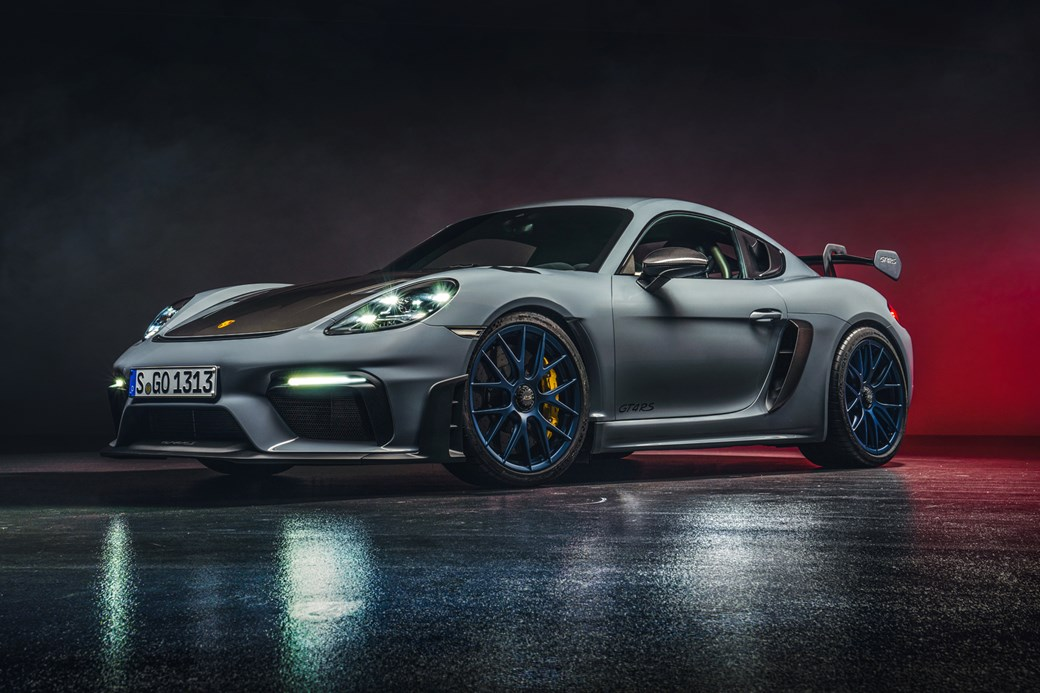
\includegraphics[width=\linewidth]{porsche_911_gt4_rs.jpg}
    \caption{An example figure}
    \label{fgr:porsche}
\end{figure}

On \autoref{fgr:porsche} you can see a Porsche 911 GT4 RS.
You can buy it on \url{https://www.porsche.com}.
\footcite{imni}

\section{table}

\begin{table}[!h]
    \centering
    \begin{tabularx}{0.5\textwidth}{XXX}
        \hline
        Alpha     & Beta     & Gamma     \\ \hline
        0         & 2        & 4         \\ \hline
        1         & 3        & 5         \\ \hline
    \end{tabularx}
    \caption{An example table}
    \label{tbl:example}
\end{table}

\begin{table}[h]
    \centering
    \begin{tabularx}{\textwidth}{lll}
        
        \hline
        \textbf{Name} & Jannis Imhof
        \\ \hline
        \textbf{Username} & imni / jimhof
        \\ \hline
        \textbf{Mail} & \href{mailto:j@imni.ch}{j@imni.ch}
        \\ \hline

    \end{tabularx}
    \caption{An other example table}
    \label{tbl:otherexample}
\end{table}


\lipsum[2-5]

\section{equations}

\begin{equation}
x_{1,2}=\frac{-b\pm\sqrt{b^2-4ac}}{2a}
\label{midnightformula}
\end{equation}

\autoref{midnightformula} is use for quadratic equations.

\begin{equation}
    i^2 = -1
\label{imaginarynumber}
\end{equation}

\autoref{imaginarynumber} is use for weird stuff.

\begin{equation}
  1 = 3 - 2
\end{equation}

\begin{align}
  f(x) &= x^2
    \\
  g(x) &= \frac{1}{x}
    \\
  F(x) &= \int^a_b \frac{1}{3}x^3
\end{align}

\begin{equation}
	\int_\alpha^\beta f'(x) \, dx=f(\beta)-f(\alpha).
\end{equation}

\[ \alpha \]
\[ \beta \]
\[ \gamma \]

We can use the fundamental theorem of calculus to say that

 $\int_2^3 x^2 \, dx=\frac{3^3}{3}-\frac{2^3}{3}=\frac{19}{3}$.  

Also note that $\displaystyle \int_2^3 x^2 \, dx=\frac{3^3}{3}-\frac{2^3}{3}=\frac{19}{3}$. 
 We can also give this equation its own line 
\[
	\int_2^3 x^2 \, dx=\frac{3^3}{3}-\frac{2^3}{3}=\frac{19}{3}.
\]

\section{code}
\begin{minted}[frame=single,framesep=10pt]{python}
import numpy as np
    
def incmatrix(genl1,genl2):
    m = len(genl1)
    n = len(genl2)
    M = None #to become the incidence matrix
    VT = np.zeros((n*m,1), int)  #dummy variable
    
    #compute the bitwise xor matrix
    M1 = bitxormatrix(genl1)
    M2 = np.triu(bitxormatrix(genl2),1) 

    for i in range(m-1):
        for j in range(i+1, m):
            [r,c] = np.where(M2 == M1[i,j])
            for k in range(len(r)):
                VT[(i)*n + r[k]] = 1;
                VT[(i)*n + c[k]] = 1;
                VT[(j)*n + r[k]] = 1;
                VT[(j)*n + c[k]] = 1;
                
                if M is None:
                    M = np.copy(VT)
                else:
                    M = np.concatenate((M, VT), 1)
                
                VT = np.zeros((n*m,1), int)
    
    return M
\end{minted}

\section{plots}
\begin{tikzpicture}
\begin{axis}[
    legend pos=outer north east,
    axis lines = center,
    xlabel = \(x\),
    ylabel = {\(f(x)\)},
    domain = -5:5,
    xmax = 5.5,
    xmin = -5.5,
    ymax = 5.5,
    ymin = -2,
    samples = 100, 
    anchor=north,
]
%Below the red parabola is defined
\addplot[color=red]{x^2 - 2*x - 1};
\addlegendentry{\(x^2 - 2x - 1\)}

%Here the blue parabola is defined
\addplot[color=blue]{x^2 + 2*x + 1};
\addlegendentry{\(x^2 + 2x + 1\)}

\end{axis}
\end{tikzpicture}


%%%%%%
\glsaddall
\printglossaries
\printbibliography[heading=bibintoc]
%%%%%%

\end{document}
